% --------------------------------------------------------------
% This is all preamble stuff that you don't have to worry about.
% Head down to where it says "Start here"
% --------------------------------------------------------------
 

% --------------------------------------------------------------
%                         Start here
% --------------------------------------------------------------
 
%\renewcommand{\qedsymbol}{\filledbox}

\title{TUTORIAL 10 - More recaps}%replace X with the appropriate number
\author{TRISTAN GLATARD\\ %replace with your name
COMP 361 Numerial Methods} %if necessary, replace with your course title
\date{November 23, 2018} 
\maketitle

\begin{exercise}{1} %You can use theorem, proposition, exercise, or reflection here. 

\begin{figure}[h]
    \centering
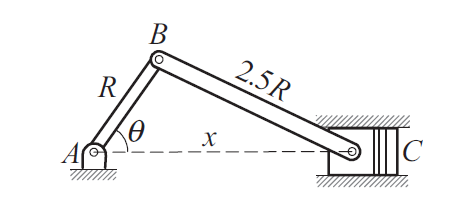
\includegraphics{5-1-12.png}
\end{figure}

The crank AB of length R = 90 mm is rotating at a constant angular speed of $d\theta/dt = 5 000$ rev/min. The position of the piston C can be shown to vary with
the angle $\theta$ as
$$x=R(cos\theta + \sqrt{2.5^2-sin^2\theta})$$
Use numerical differentiation to compute the acceleration at $\theta=0^0, 5^0, 10^0$

\textbf{Solution.} 
The acceleration is the second derivative of $x = f(\theta)= R(cos\theta + \sqrt{2.5^2-sin^2\theta})$. We will use central different approximation to calculate the acceleration at $\theta=0^0, 5^0, 10^0$ with $h=0.1$ (radian!) and $R = 0.09$ m. In this case, the approximation has the form:
$$f^{\prime\prime}(\theta) \approx \frac{f(\theta-h) -2f(\theta) + f(\theta+h)}{h^2}$$
Calculations are on the following table, note that we need to convert $\theta$ from degree to radian.

\begin{table}[h]
\centering
\begin{tabular}{|rrrrrr|}
\hline
\multicolumn{1}{|c}{\textbf{$\theta$(deg)}} & \multicolumn{1}{c}{\textbf{$\theta$(rad)}} & \multicolumn{1}{c}{\textbf{$f(\theta-h)$}} & \multicolumn{1}{c}{\textbf{$f(\theta)$}} & \multicolumn{1}{c}{\textbf{$f(\theta+h)$}} & \multicolumn{1}{c|}{\textbf{$f^{\prime\prime}(\theta)$}} \\ \hline
0 & 0.0000 & 0.3144 & 0.3150 & 0.3144 & -0.1258 \\
5 & 0.0873 & 0.3150 & 0.3145 & 0.3128 & -0.1250 \\
10 & 0.1745 & 0.3147 & 0.3131 & 0.3103 & -0.1225 \\ \hline
\end{tabular}
\end{table}

\end{exercise}

%EXERCISE 2-----------------------------------------------------
\begin{exercise}{2} %You can use theorem, proposition, exercise, or reflection here.  

The following table shows the power P supplied to the driving wheels of a car as a
function of the speed v. If the mass of the car is m = 2000 kg, determine the time
$\Delta t$ it takes for the car to accelerate from 1 m/s to 6 m/s. Use the trapezoidal rule
for integration. Hint: 	$\Delta t = m \int_{1s}^{6s}(v/P)dv$ , which can be derived from Newton’s
law $F = m(dv/dt)$ and the definition of power $P = Fv$.

\begin{table}[h]
\centering
\begin{tabular}{|c|c|c|c|c|c|c|c|c|c|c|c|}
\hline
v (m/s) & 0& 1.0& 1.8& 2.4& 3.5& 4.4& 5.1& 6.0\\ \hline
P (kW) &0 &4.7& 12.2 &19.0& 31.8& 40.1& 43.8 &43.2 \\ \hline
\end{tabular}
\end{table}

\textbf{Solution.}


Let f(v) = v/P, we transform the given table into 
\begin{table}[h]
\centering
\begin{tabular}{|c|c|c|c|c|c|c|c|c|c|c|c|}
\hline
v (m/s) & 0& 1.0& 1.8& 2.4& 3.5& 4.4& 5.1& 6.0\\ \hline
$f(v)*10^{-3}$ &0 &0.2128&	0.1475&	0.1263&	0.1101	&0.1097&0.1164	&0.1389
 \\ \hline
\end{tabular}
\end{table}

Apply trapezoidal rule on each panel,

\begin{table}[h]
\centering
\begin{tabular}{|rrrrrr|}
\hline
\multicolumn{1}{|c}{\textbf{a}} & \multicolumn{1}{c}{\textbf{b}} & \multicolumn{1}{c}{\textbf{h}} & \multicolumn{1}{c}{\textbf{$f(a)*10^{-3}$}} & \multicolumn{1}{c}{\textbf{$f(b)*10^{-3}$}} & \multicolumn{1}{c|}{\textbf{$I*10^{-3}$}} \\ \hline
1 & 1.8 & 0.8 & 0.2128 & 0.1475 & 0.14412 \\
1.8 & 2.4 & 0.6 & 0.1475 & 0.1263 & 0.08214 \\
2.4 & 3.5 & 1.1 & 0.1263 & 0.1101 & 0.13002 \\
3.5 & 4.4 & 0.9 & 0.1101 & 0.1097 & 0.09891 \\
4.4 & 5.1 & 0.7 & 0.1097 & 0.1164 & 0.079135 \\
5.1 & 6 & 0.9 & 0.1164 & 0.1389 & 0.114885 \\ \hline
\end{tabular}
\end{table}

Hence,
\begin{align}
\Delta t &= m \int_{1s}^{6s}(v/P)dv \notag \\
        &=m \int_{1s}^{6s}f(v)dv \notag \\
        &\approx \sum I \notag \\
        &=2000*0.6492*10^{-3} \notag \\
        &=1.2984 (s) \notag
\end{align}
\end{exercise}


%EXERCISE 3-----------------------------------------------------
\begin{exercise}{3} %You can use theorem, proposition, exercise, or reflection here.  

Determine $\int_1^{\infty} (1+x^4)^{-1}dx$ with the trapezoidal rule using five panels and compare
the result with the "exact" integral 0.24375. Hint: use the transformation $x^3 = 1/t$. 
\textbf{Solution.}

Let $x^3 = 1/t$, we have $dx=d(t^{-1/3})=-\frac{1}{3}t^{-4/3}dt$

The given integral becomes
\begin{align}
I&=\int_1^0 (1+t^{-4/3})^{-1}(-\frac{1}{3}t^{-4/3})dt \notag \\
&=\frac{1}{3}\int_0^1 (1+t^{4/3})^{-1}dt \notag 
\end{align}

Apply trapezoidal rule on five panels, with h = 0.2 and $f(t) = (1+t^{4/3})^{-1}$ on [0,1], we have the approximation

% Please add the following required packages to your document preamble:
% \usepackage{graphicx}
\begin{table}[h]
\centering
\begin{tabular}{|crrrrr|}
\hline
\textbf{Panel} & \multicolumn{1}{c}{$x_i$} & \multicolumn{1}{c}{$x_{i+1}$} & \multicolumn{1}{c}{$f(x_{i+1)}$} & \multicolumn{1}{c}{$f(x_{i+1})$} & \multicolumn{1}{c|}{$I_{i}$} \\ \hline
1 & 0 & 0.2 & 1.00000 & 0.89528 & 0.18953 \\
2 & 0.2 & 0.4 & 0.89528 & 0.77236 & 0.16676 \\
3 & 0.4 & 0.6 & 0.77236 & 0.66398 & 0.14363 \\
4 & 0.6 & 0.8 & 0.66398 & 0.57384 & 0.12378 \\
5 & 0.8 & 1 & 0.57384 & 0.50000 & 0.10738 \\ \hline
\end{tabular}

\end{table}

Then,
$$I = \frac{1}{3}\sum_{i=1}^{5} I_i = 0.24370$$

The result is very close to the "exact" value of 0.24375
\end{exercise}


%EXERCISE 4-----------------------------------------------------
\begin{exercise}{4} %You can use theorem, proposition, exercise, or reflection here.  
In the following sets of coupled differential equations t is the independent variable.
Convert these equations into first-order equations of the form $\dot y = F(t,y)$
\begin{enumerate}
    \item $\ddot y=x-2y$ \qquad \qquad \qquad \qquad $\ddot x = y-x$  
    \item $\ddot y=-y(\dot y^2+\dot x^2)^{1/4}$ \qquad \qquad   $\ddot x = -x(\dot y^2+\dot x^2)^{1/4}-32$  
    \item $\ddot y^2+tsiny=4\dot x$ \qquad \qquad\qquad $x\ddot x + tcosy= 4\dot y$  
\end{enumerate}

\textbf{Solution.}
Let
        $$
        y=
        \begin{bmatrix}
        y_0\\ y_1\\ y_2 \\ y_3 
        \end{bmatrix}
        =
        \begin{bmatrix}
        x\\ \dot x \\  y \\ \dot y 
        \end{bmatrix}
        $$
        
\begin{enumerate}
    \item $$
        F_1(t,y)=
        \begin{bmatrix}
        \dot y_0\\ \dot y_1\\ \dot y_2 \\ \dot y_3
        \end{bmatrix}
        =
        \begin{bmatrix}
        y_1\\ y_2-y_0 \\ y_3  \\ y_0-2y_2 
        \end{bmatrix}
        $$
    \item $$
        F_2(t,y)=
        \begin{bmatrix}
        \dot y_0\\ \dot y_1\\ \dot y_2 \\ \dot y_3
        \end{bmatrix}
        =
        \begin{bmatrix}
        y_1\\ -y_0(y_3^2+y_1^2)^{1/4}-32 \\ y_3  \\ -y_2(y_3^2+y_1^2)^{1/4}
        \end{bmatrix}
        $$
    \item $$
        F_3(t,y)=
        \begin{bmatrix}
        \dot y_0\\ \dot y_1\\ \dot y_2 \\ \dot y_3
        \end{bmatrix}
        =
        \begin{bmatrix}
        y_1\\ \frac{4y_3-tcosy_2}{y_0} \\ y_3  \\  \sqrt{4y_1-tsiny_2}
        \end{bmatrix}
        $$
\end{enumerate}

\end{exercise}

%EXERCISE 5-----------------------------------------------------
\begin{exercise}{5} %You can use theorem, proposition, exercise, or reflection here.  
Use first central difference approximations to transform the boundary value problem into simultaneous equations $Ay = b$
$$y^{\prime\prime}=y+x^2, \quad y(0)=0, \quad y(1)=1$$
\textbf{Solution.}

First central difference approximations is given as
\begin{align}
y^\prime_i &= \frac{y_{i+1}-y_{i-1}}{2h} \notag \\
y^{\prime\prime}_i &= \frac{y_{i-1}-2y_i+y_{i+1}}{h^2} \notag
\end{align}

where $h=\frac{1}{m}$ (m is to be chosen) is step size

The problem becomes
\begin{align}
\frac{y_{i-1}-2y_i+y_{i+1}}{h^2} = y_i+x_i^2,\quad i=1,2,...m-1\notag \\
y_{i-1}-2y_i+y_{i+1} - {h^2}(y_i+x_i^2) = 0, \quad i=1,2,...m-1\notag \\
y_{i-1} - (2+h^2)y_i+y_{i+1} = h^2x_i^2 , \quad i=1,2,...m-1 \label{eq1}  \notag \\
y_{i-1} - (2+\frac{1}{m^4})y_i+y_{i+1} = \frac{i^2}{m^4} , \quad i=1,2,...m-1 \end{align}

where $x_i = i*h$

The boundary conditions become
\begin{align}
y_0 &= y(x_0)= y(0) = 0 \label{eq2} \\ 
y_m &= y(x_m)= y(1) = 1 \label{eq3} 
\end{align}

Finally, we have a system of \textit{m+1} of \textit{m+1} unknowns $y_i, i=0,1,..m$ equations given by (\ref{eq1}), (\ref{eq2}) and (\ref{eq3}).

\end{exercise}


